\chapter{Deep K-Means++ Learning}
\section{Our Algorithm}
We now explain in detail  how our algorithm works. As discussed above, our goal is to learn a mapping $F:\mathcal{D}\rightarrow\mathbb{R}^d$ from the data domain $\mathcal{D}$ to an embedding space $R^d$, for some representation dimensionality $d$, such that semantically similar objects will be mapped to geometrically closer points than dissimilar objects. This will result in "naive" geometric algorithms (such as regular K-Means) to be able to cluster data correctly w.r.t a high-level similarity notion of interest. For this goal we compose a differentiable clustering module on top of a parametrized embedding module (which in our experiments we take to be a deep convolutional neural network). What's left to do then is to learn parameters for the embedding module, such that as a function, it will achieve the goal stated above.
These parameters start from some initial value, and are iteratively updated in the following way:
\begin{enumerate}
\item Sample labeled data from various different categories.
\item Embed the data with current embedding parameters.
\item Give the embedded data to the clustering module, outputing a soft partition matrix.
\item Use the Frobenius distance between the output and the ground-truth partition matrix as a loss function.
\item Calculate gradient of loss w.r.t embedding parameters.
\item Move embedding parameters in the direction opposite to this gradient.
\end{enumerate}
Let us write this more formally, in the following pseudo-code:
\begin{algorithm}[H]
\caption{Deep K-Means++ Learning}
\begin{algorithmic}[1]
	\State \textbf{Input:} Set of examples $\{\mathcal{X}_i\}_{i=1}^{M}$ from M different categories, Initial embedding parameters $\Theta_0$, Number of training steps $T$, Number $k$ of categories per train step, Size $n$ of batch per training step, Learning rates $\{\mu_i\}_{i=1}^{T}$.
    \For{i = 0 to T-1}
    	\State Sample cluster indices $\{1',..,k'\}$
        \For{j = 0 to k-1}
        	\State $X_j\gets$ Sample $\frac{n}{k}$ elements from $\mathcal{X}_{j'}$
        \EndFor
        \State $Y\gets \begin{bmatrix}
    1_{\frac{n}{k},\frac{n}{k}} & 0 & \dots & 0 \\
    0 & 1_{\frac{n}{k},\frac{n}{k}} & \dots & 0\\
    \vdots & \vdots & \ddots & \vdots \\
    0 & 0 & \dots & 1_{\frac{n}{k},\frac{n}{k}}
	\end{bmatrix} _{n,n}$ \Comment{ground-truth clustering matrix}
        \State $X \gets [X_1,X_2,..,X_k]$ 
        \State $\widetilde{X} \leftarrow$ Embed($X,\Theta_i$) \Comment{data embeddings}
  		\State $\widetilde{Y} \leftarrow$ Deep K-Means++($\widetilde{X}$,k) \Comment{inferred clustering matrix}
        \State $loss \gets \left\lVert Y-\widetilde{Y} \right\rVert ^{2}$ \Comment{Frobenius norm of matrix differences}
        \State $\Theta_{i+1} \gets \Theta_i - \mu_i \frac{\partial loss}{\partial \Theta_i}$ \Comment{gradient descent} % todo: define mu
    \EndFor
    \State \Return $\Theta_T$
\end{algorithmic}
\end{algorithm}

At lines 3-5, we sample a sub-problem, by sampling a small number of clusters and data points therefrom. The ground-truth "label" for this sub-problem is simply the block diagonal matrix shown in the pseudo-code. 
What's left to describe is the operation of the functions called at lines 8 and 9. Line 8 includes a call to the embedding module $Embed$, which should generally be a domain-dependent function. In our empirical evaluations over images, we take $Embed$ to be a deep convolutional neural network. In our synthetic experiments, we take it to be a simple linear mapping.
Line 9 includes the call to the clustering module. As discussed above, this module is a differentiable formulation of the K-Means++ algorithm. Section \ref{diff_clust} in the current chapter describes this module in detail.
\subsubsection{Sub-Problem Gradients}
Our training regime works by sampling "clustering sub-problems". We sample uniformly $\frac{n}{k}$ data points from $k$ uniformly sampled clusters, and define the loss to be the Frobenius distance between the ground-truth partition matrix and the our clustering module's output matrix. Performing gradient descent w.r.t a loss defined over a random sample of data is a common practice in contemporary large-scale settings, where the data simply cannot fit altogether inside a single GPU/RAM. 
In most supervised learning scenarios though, there is a supervision signal associated with each data point individually, and the loss function over the data $L(X,Y;\Theta)$ is defined as an average of pointwise losses $\frac{1}{n}\sum_{i\in [n]} L(x_i,y_i;\Theta)$. In such scenarios, if the "sub-problems" are sampled uniformly, the training regime is known as Stochastic Gradient Descent, and the gradient of the loss over the sub-problems is, as a random variable, an unbiased estimator for the gradient of the empirical risk in general.
In the case of clustering, it's not immediate to see how an "empirical clustering risk" should be defined. Let us say we define it as how well was the entire data set jointly clustered. If using the Frobenius metric, this can formalized as: 
\begin{equation}
L_A(X,Y;\Theta) = \expect{A}{||A(X;\Theta) - Y ||^2}
\end{equation}
Where $A$ is the clustering algorithm, and the expectation is taken w.r.t it's randomness. The output of $A$ is an $nxn$ (possibly soft) partition matrix.
Since it is meaningless to cluster a single point, this empirical loss doesn't decompose to an average pointwise losses. Still, one might ask if the gradients for clustering sub-problems forms an unbiased estimator for the gradient of the empirical risk in general. Our simulations suggest that at least for the Frobenius norm, this is not necessarily the case. 
\begin{comment}
Example with sym hexagon.
\end{comment}

\section{Differentiable K-Means Clustering}
\label{diff_clust}
\subsection{The K-Means Objective}
The clustering module searches iteratively for (locally) optimal centroids and beliefs $C\in \reals^{k,d},B\in\reals^{n,k}$ w.r.t the relaxed K-Means objective:
\begin{equation*}
\begin{aligned}
& \underset{C\in \reals^{k,d},B\in\reals^{n,k}}{\text{minimize}}
& & ||C-B\widetilde{X}||^2 \\
& \text{subject to:}
& & \forall i\in\{1,...,n\}: B_i \in \Delta_k \text{ (i'th row of B is a distribution)}
\end{aligned}
\end{equation*}
Where $\widetilde{X}$ is the embedded data matrix.
Intuitively, an optimum for this objective seeks to find a clustering such that data points are close to their cluster's mean.
In the integral formulation of this optimization problem, i.e when $B\in \{M\in\{0,1\}^{n,k}|M\vec{1}_k = \vec{1}_n\}$, the optimum corresponds to a clustering which minimizes intra-cluster sum of squares $\sum_{i=1}^{k}\sum_{x\in S_i}{||x-\mu_i||^2}$, where $S_i$ is the $i$'th cluster, and $\mu_i$ is the $i$'th cluster's mean.
It is well-known that optimizing the integral version is NP-hard. In fact, it is NP-hard even for $k=2$ clusters (when dimensionality $d$ is taken as a parameter), and even so when $d=2$, for a general number of clusters.
Using a relaxed formulation is a common approach to derive an approximation algorithm. In chapter \ref{chap:Related_Work} we mention several of these approaches in the context of learning a metric for data.
Another common approach is to use what is known as Loyd's algorithm ( also known as Voronoi iterations), and to "bootstrap" $B$ and $C$, starting from some initialization. It is much simpler to describe these iterations when switching from the matrix variables $B$, and using instead the variable $\{S_i\}_{i=1}^{k}$, where the set $S_i$ is the $i$'th cluster. This switch is possible only since we are dealing with the integral formulation, and the rows of the $B$ matrix in this case are all $k$-dimensional one-hot vectors, which serve as indicators. I.e, the $j$'th row indicates to which cluster is the $j$'th datapoint assigned to. 
We use $C_i$ to denote the centroid of the $i$'th.
Loyd's algorithm's update steps are thus the following:
\begin{equation*} 
\begin{aligned}
& S_{i}^{(t+1)}= \{X_p : ||X_p-C_{i}^{(t)}||^2\leq||X_p-C_{j}^{(t)}||^2 \quad \forall j\in[k] \} \\
& C_{i}^{(t+1)}= \frac{1}{|S_i^{(t+1)}|}\sum_{X_p\in S_i^{(t+1)}}{X_p}
\end{aligned}
\end{equation*}
Each iteration updates one of the variables $S,C$ in a way which is optimal w.r.t the other variable. Thus the objective is non-increasing as iterations progress.
In simple terms, the cluster membership updates corresponds to assigning each point to the cluster whose centroid is nearest, and the centroid updates correspond to having each cluster's centroid to be it's vector mean.
In Loyd's original algorithm these bootstraping continues until a fixed-point has been reached. Since each step decreases the objective, this fixed-point will be a local optimum. 
From NP-hardness of the problem, the initialization scheme (i.e choice of initial centroids) is crucial for performance. Arbitrary initializations can result in convergence to a local optimum arbitrarily worse than the global optimum. Despite this, there are initialization schemes under which there are proven bounds for approximation ratio, i.e how far the result on convergence will be from an optimal one. One of these initialization schemes is K-Means++'s initialization, which will be detailed later on this chapter. 
Let us first discuss our differentiable formulation of the above update steps.
\subsection{Differentiable K-Means Iterations}
\begin{figure}[h!]
\centering
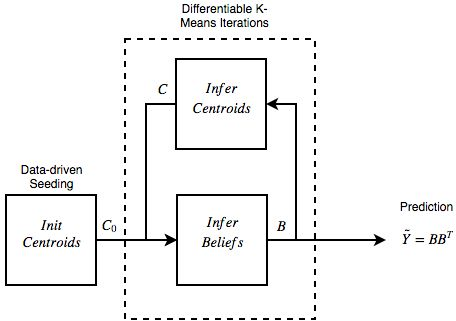
\includegraphics[width=0.7\textwidth]{imgs/dkmpp.jpg}
\caption{\label{fig:frog}Block diagram for clustering module.}
\end{figure}
As recalled, the original purpose of our algorithm was to learn parameters for an embedding function, s.t data embedded under it will yield good clustering performance, when clustered via algorithms which seek to minimize the K-Means objective. For this end we need the clustering inference to be a differentiable function, so that gradients could be back-propagated.
Let us notice that in Loyd's algorithm, the only part in the update steps which isn't differentiable is the assignment of datapoints to clusters, for which an $argmin$ needs to be computed. This operation is clearly not differentiable, and so instead we propose to use a $softmin$. This operation turns our assignments into soft-decisions, which we denote as beliefs, and represent via a row-stochastic belief matrix $B\in \reals^{n,k}$
The equations for the relaxed Voronoi updates are, in matrix notation: 
\begin{equation*} 
\begin{aligned}
& B_{t+1} = softmin(dist\_mat(X,C_{t})) \\
& C_{t+1} = diag((B_{t+1}^T X)\vec{1} )^{-1}(B_{t+1}^T X)
\end{aligned}
\end{equation*}
Where $dist_mat$ is defined as.. TODO 
,and $diag$ is defined by taking a vector as input, and giving a square matrix whose main diagonal is that vector as output.
For further clarity, let us view these updates in pseudo-code and describe the meaning of each line:
%todo: change name to deep expectation maximization
\begin{algorithm}[H]
\caption{Deep K-Means++}
\begin{algorithmic}[1]
	\State \textbf{Input:} Embedded Data $\widetilde{X}$, Number of clusters $k$, Unroll depth $l$. 
    \State $C_0 \gets $ Deep K-Means++ Init($\widetilde{X}$) \Comment{Data-driven centroid initialization}
    \For{i = 1 to l}
    \State $B_i \gets $ Infer-Beliefs($\widetilde{X},C_{i-1},\beta$)
    \State $C_i \gets $ Infer-Centroids($\widetilde{X},B_{i-1}$)
    \EndFor
    \State \Return $B_{l} B_{l}^{T}$
\end{algorithmic}
\end{algorithm}
\begin{algorithm}[H]
\caption{Get Distance Matrix}
\begin{algorithmic}[1]
	\State \textbf{Input:} Two matrices $A\in\mathbb{R}_{n,d},B\in\mathbb{R}_{k,d}$, with same row dimensionality
    \State $D \gets (A\odot A)1_{d,k}-2AB^{T}+((B\odot B)1_{d,k})^{T}$ \Comment{Using lin. alg. identity: $||u-v||^2=||u||^2-2<u,v>+||v||^2$}
    \State Return $D$ \Comment{$ij$'th cell stores squared euclidean distance between $i$'th row of $A$ and $j$'th row of $B$}
\end{algorithmic}
\end{algorithm}
\begin{minipage}[t]{8cm}
  \vspace{0pt}  
  \begin{algorithm}[H]
    \caption{Infer-Beliefs}
    \begin{algorithmic}[1]
    \State \textbf{Input:} Data Matrix $X$, Centroid Matrix $C$
    \State $dist\_mat \gets get\_distance\_matrix(X,C)$
    \State \Return $softmin(dist\_mat)$
    \end{algorithmic}
  \end{algorithm}
\end{minipage}%
\begin{minipage}[t]{7cm}
  \vspace{0pt}
  \begin{algorithm}[H]
    \caption{Infer-Centroids}
    \begin{algorithmic}[1]
    \State \textbf{Input:} Data Matrix $X$, Belief Matrix $B$
    \State $cluster\_sums \gets B^T X $
    \State $cluster\_sizes \gets cluster\_sums\dot\vec{1} $
    \State $normalizer \gets diag(cluster\_sums)^{-1}$
    \State \Return $ normalizer\times{cluster\_sums}$
    \end{algorithmic}
  \end{algorithm}
  
\end{minipage}


The clustering module's pseudo-code is described at algorithm 2, and is based on a differentiable formulation of the K-Means++ algorithm. As mentioned above,

This clustering module represents the clustering using a set of underlying cluster centroids, which induce the soft-assignment (which we will denote by the term beliefs) of data points to clusters. The belief vector for each data point is given by applying a softmin operation over the vector of euclidean distances between that data point and the existing centroids. We use a softmin instead of an actual argmin so that our cluster inference will be a differentiable function, and will thus yield to end-to-end gradient descent updates.

\section{Differentiable Centroid Sampling}
for the gradient signal to be helpful, we need the clustering inference to work properly. If the data is embedded correctly, i.e such the the global optimal cluster
In order for the learning process not to be derailed by wrong clusterings (i.e, the gradient update will move the embedding parameters in a direction such that the labeled data will be better clustered under a bad local minima in the clustering output space)
\begin{algorithm}[H]
\caption{Deep K-Means++ Init}
\begin{algorithmic}[1]
	\State \textbf{Input:} Data matrix $X$, Number of desired clusters $k$.
    %\bindent
    \State $C_0 \gets X_0$ \Comment{assign first centroid to be arbitrary data point}
    \For{i = 1 to k-1}
    	\State $C \gets [C_0,..,C_{i-1}]$
    	\State $D \gets get\_dist\_mat(X,C)$ \Comment{ $ij$'th cell stores squared euclidean distance between $i$'th data point and $j$'th centroid}
        \State $\widetilde{D} \gets softmin(D)\odot D$ \Comment{apply softmin over every row, and multiply element-wise with $D$ }
    	\State $\pi \gets \frac{\widetilde{D}\vec{1_{i}}}{\vec{1_{n}}\widetilde{D}\vec{1_{i}}}$ \Comment{sum over rows and normalize. $\pi$ thus represents a discrete distribution}
    	\State $\vec{q} \gets gumbel\_softmax\_sampling(\pi)$ \Comment{relaxed one-hot vector indicating $i$th centroid picked} 
    	\State $C_i \gets \vec{q}X$
    \EndFor
    \State $C \gets [C_0,..,C_{k-1}]$
	\State \Return $C$
	%\eindent
\end{algorithmic}
\end{algorithm}
We now describe how we implement {\it{k-means++}}'s centroid initialization as a differentiable layer in a neural network.\\
As in {\it{k-means++}} our algorithm proposes centroids iteratively. At the first iteration, we simply propose an arbitrary data point. At the $t+1$'th iteration, $t$ centroids, denoted as $\{c_i\}_{i=1}^{t}$, have already been proposed. 
A matrix $D$ of size $[n,t]$ can thus be built, such that $A_{i,j} =  ||x_i-c_j||^2$. By taking a soft-min over $D$'s rows and normalizing the result to 1, we have an approximation for the probability vector, whose $i$'th entry is  \\
\subsection{Gumbel-Softmax Sampling}
%explanation of gumbel softmax sampling. gumbel distribution, etc
Gumbel-Softmax Sampling is a differentiable version of sampling from a discrete probability distribution. This technique allows defining neural networks with layers that act as discrete samplers. 
TODO: add when this is usefull (gans,etc..)
Notice that it is not possible to implement such layers in neural networks without any output smoothing, since sampling from a discrete distribution is inherently non-differentiable.\\
The sampling layer takes as input a vector of probabilities $\{p_i\}_{i=1}^{n}$, and outputs a distribution over possible 

The method uses the following key fact from probability theory:
\begin{thm}
(Gumbel Sampling) Let $p_1,...,p_n \in \Delta_n$ be $n$ numbers on the $n$-simplex, and denote by $D$ a random variable over $[n]$, distributed by $P[D=i]=p_i$.\\
Let $Z$ be a random variable over $\reals$ with the following probability density function: $f(z) = e^{-z+e^{-z}}$.\\
Then, the random variable $argmax_{i\in[n]}\{Z\cdot p_i\}$ has the same distribution as $D$.
\end{thm}
\begin{proof} 
Let $\{x_i\}_{i=1}^{n}$ be $n$ real numbers s.t $\forall i\in[n]: p_{i} = \frac{e^x_i}{\sum_{k'}}$
\end{proof}
\begin{algorithm}[H]
\caption{Gumbel-Softmax Sampling}
\begin{algorithmic}[1]
	\State \textbf{Input:} A discrete probability distribution $\pi = \{p_i\}_{i=1}^{n}$
    %\bindent
    \State sample $\vec{z}\in \mathbb{R}^n$, where each coordinate is sampled according to the Gumbel distribution: $p(z) = e^{-(z+e^{-z})}$
    \State $\widetilde{\pi} \gets \pi \odot \vec{z}$ \Comment{multiplicatively perturbed values}
    \State Return $softmax(\widetilde{\pi})$
    %\eindent
\end{algorithmic}
\end{algorithm}